%Version 2.1 April 2023
% See section 11 of the User Manual for version history
%
%%%%%%%%%%%%%%%%%%%%%%%%%%%%%%%%%%%%%%%%%%%%%%%%%%%%%%%%%%%%%%%%%%%%%%
%%                                                                 %%
%% Please do not use \input{...} to include other tex files.       %%
%% Submit your LaTeX manuscript as one .tex document.              %%
%%                                                                 %%
%% All additional figures and files should be attached             %%
%% separately and not embedded in the \TeX\ document itself.       %%
%%                                                                 %%
%%%%%%%%%%%%%%%%%%%%%%%%%%%%%%%%%%%%%%%%%%%%%%%%%%%%%%%%%%%%%%%%%%%%%

%%\documentclass[referee,sn-basic]{sn-jnl}% referee option is meant for double line spacing

%%=======================================================%%
%% to print line numbers in the margin use lineno option %%
%%=======================================================%%

%%\documentclass[lineno,sn-basic]{sn-jnl}% Basic Springer Nature Reference Style/Chemistry Reference Style

%%======================================================%%
%% to compile with pdflatex/xelatex use pdflatex option %%
%%======================================================%%

%%\documentclass[pdflatex,sn-basic]{sn-jnl}% Basic Springer Nature Reference Style/Chemistry Reference Style


%%Note: the following reference styles support Namedate and Numbered referencing. By default the style follows the most common style. To switch between the options you can add or remove “Numbered” in the optional parenthesis. 
%%The option is available for: sn-basic.bst, sn-vancouver.bst, sn-chicago.bst, sn-mathphys.bst. %  
 
%%\documentclass[sn-nature]{sn-jnl}% Style for submissions to Nature Portfolio journals
%%\documentclass[sn-basic]{sn-jnl}% Basic Springer Nature Reference Style/Chemistry Reference Style
\documentclass[sn-mathphys,Numbered]{sn-jnl}% Math and Physical Sciences Reference Style
%%\documentclass[sn-aps]{sn-jnl}% American Physical Society (APS) Reference Style
%%\documentclass[sn-vancouver,Numbered]{sn-jnl}% Vancouver Reference Style
%%\documentclass[sn-apa]{sn-jnl}% APA Reference Style 
%%\documentclass[sn-chicago]{sn-jnl}% Chicago-based Humanities Reference Style
%%\documentclass[default]{sn-jnl}% Default
%%\documentclass[default,iicol]{sn-jnl}% Default with double column layout

%%%% Standard Packages
%%<additional latex packages if required can be included here>
\usepackage[T1]{fontenc}
\usepackage{graphicx}%
\usepackage{multirow}%
\usepackage[table,xcdraw]{xcolor}
\usepackage{amsmath,amssymb,amsfonts}%
\usepackage{amsthm}%
\usepackage[gen]{eurosym}
\usepackage{mathrsfs}%
\usepackage[title]{appendix}%
\usepackage{xcolor}%
\usepackage{textcomp}%
\usepackage{manyfoot}%
\usepackage{booktabs}%
\usepackage{algorithm}%
\usepackage{algorithmicx}%
\usepackage{algpseudocode}%
\usepackage{listings}%
\usepackage{orcidlink}
%%%%

%%%%%=============================================================================%%%%
%%%%  Remarks: This template is provided to aid authors with the preparation
%%%%  of original research articles intended for submission to journals published 
%%%%  by Springer Nature. The guidance has been prepared in partnership with 
%%%%  production teams to conform to Springer Nature technical requirements. 
%%%%  Editorial and presentation requirements differ among journal portfolios and 
%%%%  research disciplines. You may find sections in this template are irrelevant 
%%%%  to your work and are empowered to omit any such section if allowed by the 
%%%%  journal you intend to submit to. The submission guidelines and policies 
%%%%  of the journal take precedence. A detailed User Manual is available in the 
%%%%  template package for technical guidance.
%%%%%=============================================================================%%%%

%\jyear{2021}%

\begin{document}

\title[Bayesian optimization with additive kernels for a stepwise calibration of simulation models for cost-effectiveness analysis]{Bayesian optimization with additive kernels for a stepwise calibration of simulation models for cost-effectiveness analysis}

\def\thefootnote{}\footnotetext{This article is an extension of the work presented at CCIA 2023\cite{original}}

%%=============================================================%%
%% Prefix	-> \pfx{Dr}
%% GivenName	-> \fnm{Joergen W.}
%% Particle	-> \spfx{van der} -> surname prefix
%% FamilyName	-> \sur{Ploeg}
%% Suffix	-> \sfx{IV}
%% NatureName	-> \tanm{Poet Laureate} -> Title after name
%% Degrees	-> \dgr{MSc, PhD}
%% \author*[1,2]{\pfx{Dr} \fnm{Joergen W.} \spfx{van der} \sur{Ploeg} \sfx{IV} \tanm{Poet Laureate} 
%%                 \dgr{MSc, PhD}}\email{iauthor@gmail.com}
%%=============================================================%%

\author*[1,2]{\fnm{David} \sur{Gómez-Guillén}\orcidlink{0000-0003-1787-6482}}\email{dgomez@iconcologia.net}
\author[2,3]{\fnm{Mireia} \sur{Díaz}\orcidlink{0000-0001-9360-4548}}\email{mireia@iconcologia.net}
\author[4]{\fnm{Josep Lluís} \sur{Arcos}\orcidlink{0000-0001-7751-1210}}\email{arcos@iiia.csic.es}
\author[4]{\fnm{Jesus} \sur{Cerquides}\orcidlink{0000-0002-3752-644X}}\email{cerquide@iiia.csic.es}

\affil*[1]{Universitat Autònoma de Barcelona (UAB), \city{Bellaterra}, \country{Spain}}
\affil[2]{Institut Català d'Oncologia (ICO) - Institut d'Investigació Biomèdica de Bellvitge (IDIBELL), \city{Hospitalet de Llobregat}, \country{Spain}}
\affil[3]{Consortium for Biomedical Research in Epidemiology and Public Health - CIBERESP. Carlos III Institute of Health, \city{Madrid}, \country{Spain}}
\affil[4]{Institut d'Investigació en Intel·ligència Artificial - Consell Superior d'Investigacions Científiques (IIIA-CSIC), \city{Bellaterra}, \country{Spain}}


%%==================================%%
%% sample for unstructured abstract %%
%%==================================%%

\abstract{The use of mathematical simulation models of diseases in economic evaluation is an essential and common tool in medicine aimed at guiding decision-making in health. Cost-effectiveness analyses are a type of economic evaluation that assess the balance between health benefits and the economic sustainability of different health interventions, often with the use of mathematical models. One critical aspect of these models is the accurate representation of the disease's natural history, which requires a set of parameters such as probabilities and disease burden rates. While these parameters can be obtained from scientific literature, they often need calibration to fit the model's expected outcomes. However, the calibration process can be computationally expensive and traditional optimization methods can be time-consuming due to relatively simple heuristics that may not even guarantee feasible solutions.
	
In this work, we investigate the use of Bayesian optimization to enhance the calibration process by leveraging domain-specific knowledge and exploiting structural properties in the solution space. Specifically, we examine the effect of additive kernel decomposition and the use of a stepwise approach that exploits the sequential block structure in simulation models to break down a large optimization problem into several smaller problems without sacrificing the quality of the solutions. In some cases the parameters obtained might even have less error over those found by conventional calibration.
	
Our preliminary results show that a Bayesian optimization procedure asymptotically improves the calibration process, leading to faster convergence and better solutions for larger simulation models, especially when paired with a stepwise calibration methodology.}


\keywords{bayesian optimization, gaussian processes, additive kernels, model calibration, simulation models, cancer research}

\maketitle

\section{Introduction}\label{sec1}

Healthcare interventions are increasingly being evaluated based on their cost-effectiveness due to usual budgetary constraints, ensuring equitable and efficient distribution of healthcare services. These constraints mean that not all available and effective interventions can be included in health plans. In many countries, it has become standard policy to assess the costs of new healthcare interventions in relation to their expected benefits before implementing them. Cost-effectiveness analysis (CEA) using mathematical simulation models is a crucial tool in this context, enabling us to assess the value of healthcare interventions and determine which ones offer the best value for money\cite{drummond}. By comparing the costs and benefits of alternative interventions, policymakers and healthcare providers can prioritize strategies and allocate resources to achieve the maximum health benefits for the population. Ultimately, the goal of healthcare is to improve health outcomes, and CEA plays a vital role in achieving this objective\cite{levin}.

CEA usually relies on simulation models that mimic disease processes to project the effects of different medical strategies on health outcomes over time\cite{applied_he}. There are different types of models but some of the most common simulate the traversal of a group of individuals through different health states (figure \ref{fig:lung_model}). These models can generate various outcomes, such as the average cost and the average life expectancy, usually measured in Quality-Adjusted Life Years (QALYs)\cite{qalys}.

\begin{figure}[h!]
	\centering	
	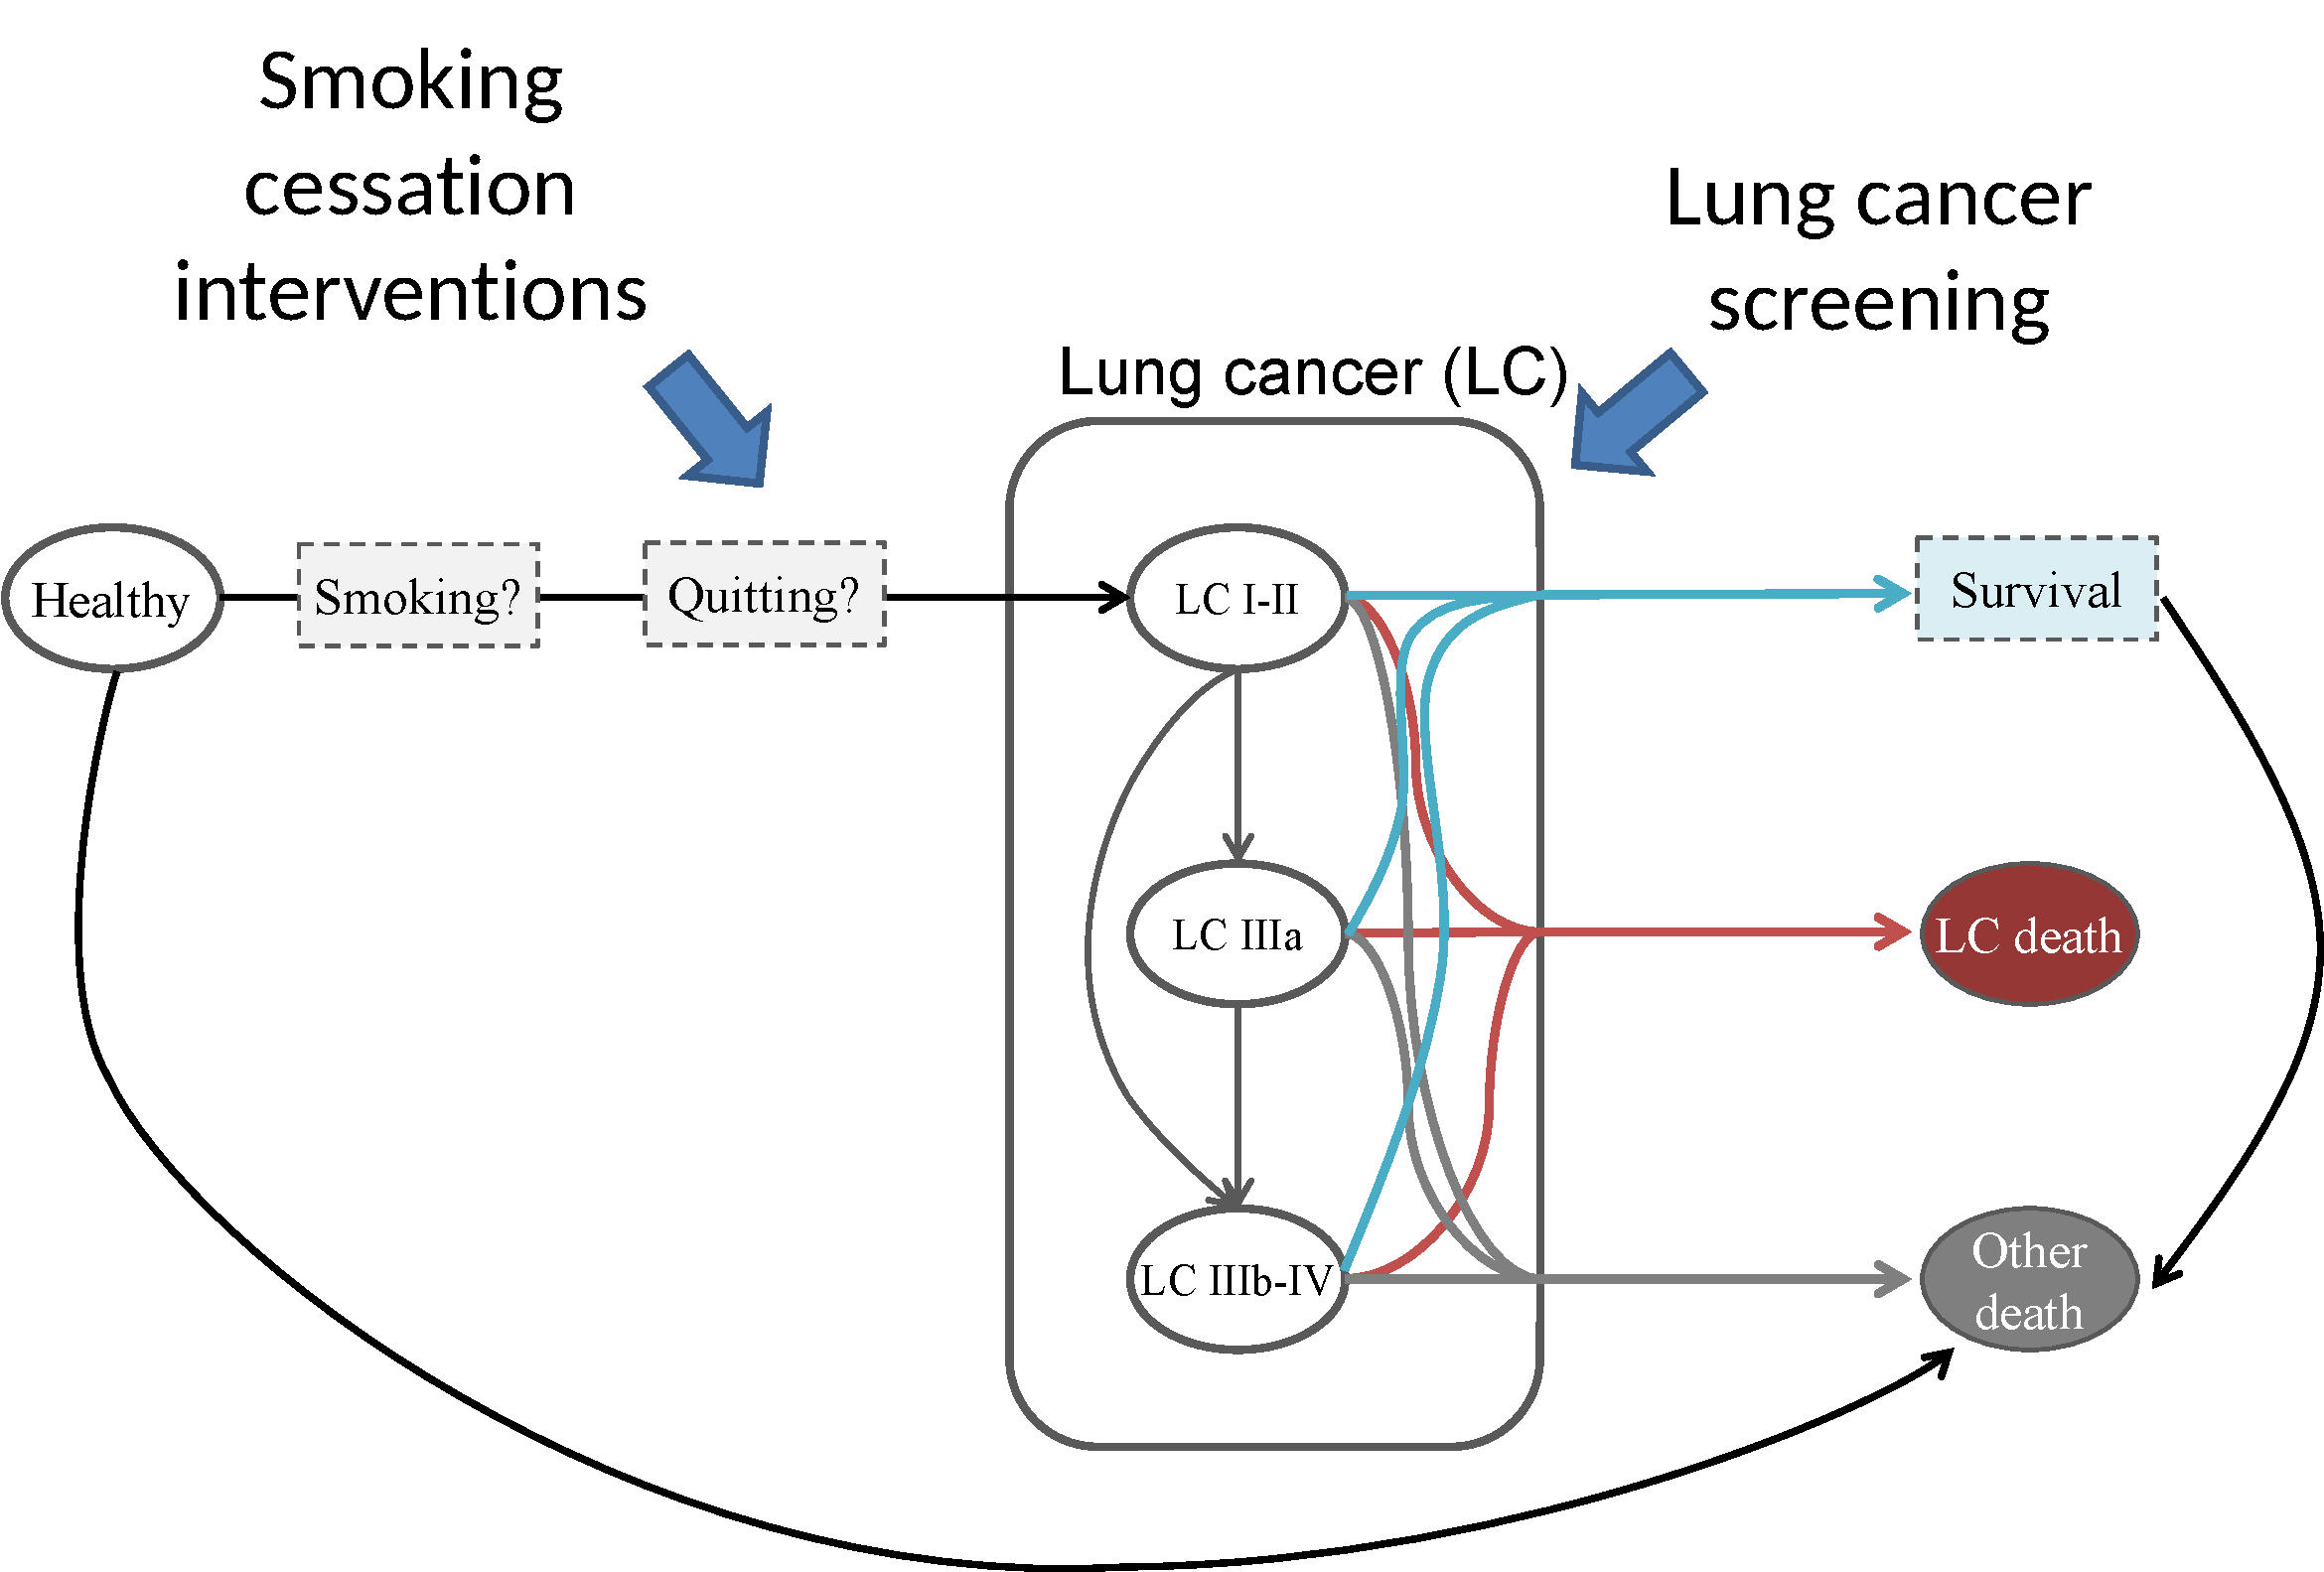
\includegraphics[width=80mm]{figs/lungmodel.pdf}		
	\caption{Lung cancer markov model state diagram}	
	\label{fig:lung_model}	
\end{figure}

In order to execute the simulations, input parameters are required to describe the disease process, such as probabilities, hazard ratios, or disease burden rates extracted from scientific literature. Due to the inherent uncertainty of these values, it is often necessary to calibrate the model before proceeding with the analysis. Calibration consists in adjusting the input parameters until the resulting output approximates a target value identified in the scientific literature, such as disease incidence, prevalence, or mortality. This optimization process can be especially taxing for complex models, and may necessitate the use of advanced techniques to efficiently explore the solution space.

Moreover, calibrations can be highly dimensional optimization problems with many arbitrary constraints between parameters, dictated by the specific medical domain. In this work, we explore the challenges associated with calibrating simulation models and propose methods to overcome them. Our research provides valuable insight into novel ways to calibrate these simulation models more efficiently using Bayesian Optimization. We also investigate the circumstances under which it outperforms common methods used in the field.	

\section{Background}

\subsection{Bayesian Optimization}

Bayesian optimization is a powerful technique for optimizing expensive, black-box functions that are difficult or time-consuming to evaluate. The basic idea is to build a probabilistic model of the function based on the observations made so far, and then use this model to guide the selection of new points to evaluate. The method is particularly useful when the objective function is complex and has multiple input variables.

At the heart of Bayesian optimization is a probabilistic model, typically a Gaussian process, that captures the beliefs about the unknown function we are trying to optimize. The GP provides a distribution over functions that is consistent with the observed data, and allows us to reason about the uncertainty associated with our predictions. We start by selecting a few initial points to evaluate, and use these to fit the GP model. We then iteratively select new points to evaluate based on a trade-off between exploration (trying to find regions of the input space with high uncertainty) and exploitation (trying to find regions with high predicted performance).

The key advantage of Bayesian optimization is that it can find the global optimum of the function with relatively few evaluations, even in high-dimensional spaces. This is because the method actively seeks out the most promising areas of the input space to evaluate next, rather than simply evaluating points at random. The downside is that the method can be computationally expensive, especially for functions with a large number of input variables or when the GP model is complex.

Bayesian optimization has been successfully applied to a wide range of optimization problems in machine learning, including hyperparameter tuning, experimental design, and automatic algorithm configuration. In these applications, the objective function is often a performance metric that is expensive to evaluate, such as the validation error of a machine learning model. Bayesian optimization can help to quickly identify good values of the hyperparameters or experimental conditions, without having to exhaustively search the entire parameter space.

\subsection{Gaussian Processes}
Gaussian Processes (GPs) are non-parametric regression models that represent each observation as a random variable drawn from a Gaussian distribution $f(x) \sim \mathcal{N}(\mu(x), k(x,x))$\cite{gaussian-processes}. The mean function $\mu(x)$ and the covariance function $k(x,x')$ define the expected value of the Gaussian Process and the degree of dissimilarity between different inputs, respectively. For an assumed noise level in the data $\sigma^2$, an initial prior $\mu_0(X)$ (often $\mu_0(X)=0$), a given observation set $X=\{\vec{x_1}, ..., \vec{x_D}\}$ with labels $\vec{y}$ and a Gram matrix $K$ built from $X$ and a set of unknown observations $X_*$, a Gaussian Process $f_*$ has an analytic form for the predictive posterior distribution (equation \ref{eq:predictive_posterior}).

\begin{equation} \label{eq:predictive_posterior}
	\begin{aligned}
		f_*|X,\vec{y},X_* & \sim \mathcal{N}(\mu(X_*), \Sigma(X_*)) \\
		\mu(X_*) & = \mu_0(X_*) + K(X_*,X)(K(X,X) + \sigma^2 I)^{-1}(\vec{y} - \mu_0(X_*)) \\
		\Sigma(X_*) & = K(X_*,X_*) + \sigma^2 I - K(X_*,X)(K(X,X) + \sigma^2 I)^{-1} K(X,X_*)
	\end{aligned}
\end{equation}	

The covariance function or kernel is the mechanism to give a Gaussian Process its expressive power, and its choice will heavily depend on the kind of function we aim to model\cite{kernel-composition}. The squared exponential (SE) kernel $k(x,x') = \sigma^2 e^{-\frac{||x-x'||^2}{2l^2}}$ is a popular choice, despite significant drawbacks such as its locality and sensitivity to the curse of dimensionality\cite{curse-dimensionality}.
In general, modeling complex high dimensional functions using a single kernel can be computationally expensive using local kernels, making this a first class research problem (e.g. \cite{gp-high-dim}\cite{gp-high-dim2}).

Additive kernel decomposition\cite{gp-additive} addresses this problem by breaking down the kernel into a sum of simpler kernels, each of which captures a different aspect of the relationship between the input variables. This approach can capture both local and global interactions between the input variables. Additionally, additive kernel decomposition can improve the interpretability of the model, as each kernel term can be associated with a specific interaction term. This can help users understand which orders of interaction are important for the current optimization problem. 

Additive kernels suffer from the non-identifiability problem: the kernel hyperparameters are not uniquely identifiable from the observed data, which can lead to challenges in model selection and interpretation.
To ensure a unique decomposition, Lu et al\cite{gp-additive-orthogonal} proposed an extension of additive kernels by including an extra constant kernel $\tilde{k}_{add_0}(x,x')$ with an additional variance hyperparameter $\sigma_0^2$ and an orthogonality constraint to generate Orthogonal Additive Kernels (OAK)\cite{gp-additive-orthogonal}. Assuming a normal input distribution $x_i \sim \mathcal{N}(\mu_i, \delta_i^2)$, the following constrained base kernel is derived:

\begin{equation} \label{eq:additive-orthogonal}
	\begin{aligned}
		k_{add_{OAK}}(x,x') &= \sum_{i=0}^D{\sigma_i^2  \tilde{k}_{add_i}(x_i,x_i')} \\
		%\tilde{k}_{add_0}(x,x') &= 1\\
		\tilde{k}_{add_j}(x,x') &= \sum_{1\leq i_1 < i_2 < \ldots < i_j\leq D} \left[\prod_{d=1}^{j} \tilde{k}_{i_d}(x_{i_d},x_{i_d}') \right]\\		
		\tilde{k}_i(x,x') &= e^{\frac{(x_i-x_i')^2}{2l_i^2}} - \frac{l_i\sqrt{l_i^2 + 2\delta_i^2}}{l_i^2 + \delta_i^2} e^{-\frac{(x_i-\mu_i)^2 + (x_i'-\mu_i)^2}{2(l_i^2 + \delta_i^2)}}
	\end{aligned}
\end{equation}

One important advantage of these additive kernels is that we can interpret the $\sigma_i^2$ as the contribution of each individual order to the total kernel. Since many problems often rely on a few low-order interactions, we can truncate the higher orders and limit the computational cost while retaining most of the information present in the full decomposition. To achieve this, OAK can be useful to accurately identify each contribution and provide an accurate representation on the actual composition on the function.

In this document, the BO method using Gaussian processes with a SE kernel will be referred to as BO-SE, while the same method using OAK will be called BO-OAK.

\section{Methodology}
In this section we will describe the simulation model and the optimization methods we will use to calibrate it.

\subsection{Simulation Model}
\label{sec:simulation-model}
We use a lung cancer model presented in a published cost-effectiveness analysis\cite{lung-model} as a fast benchmark for Bayesian Optimization on simulation models. This Markov-based microsimulation model simulates a cohort's progression through seven different health states over time. The transition probabilities used in the model were age-specific, with distinct values for each 5-year age group (35-39, 40-44, ..., 75-79). The state diagram for this model is pictured in figure \ref{fig:lung_model}.

To simplify the calibration tests, certain simulation details such as gender differentiation, smoking prevalence or quitting probabilities for smokers were ignored. Certain inherent constraints, such as ensuring that the sum of the probabilities in each row equals one or that certain probabilities are zero, were imposed on the matrices. This allowed the number of parameters to be optimized per age group to be reduced from 36 to 11. Furthermore, this model was designed to be computationally inexpensive, taking less than 10ms to simulate. By introducing arbitrary delays in the model we can observe the relationship between calibration times and model simulation times and extrapolate the results for more time-consuming models.

The calibration target for the model was defined as the weighted sum of the euclidean distances between the observed and expected outputs of interest, namely lung cancer incidence (45\%), lung cancer mortality (45\%) and mortality from other causes (10\%), computed for each age group. An example of these calibrations is illustrated in figure \ref{fig:calibration-curve}.

\begin{figure}[h!]
	\centering	
	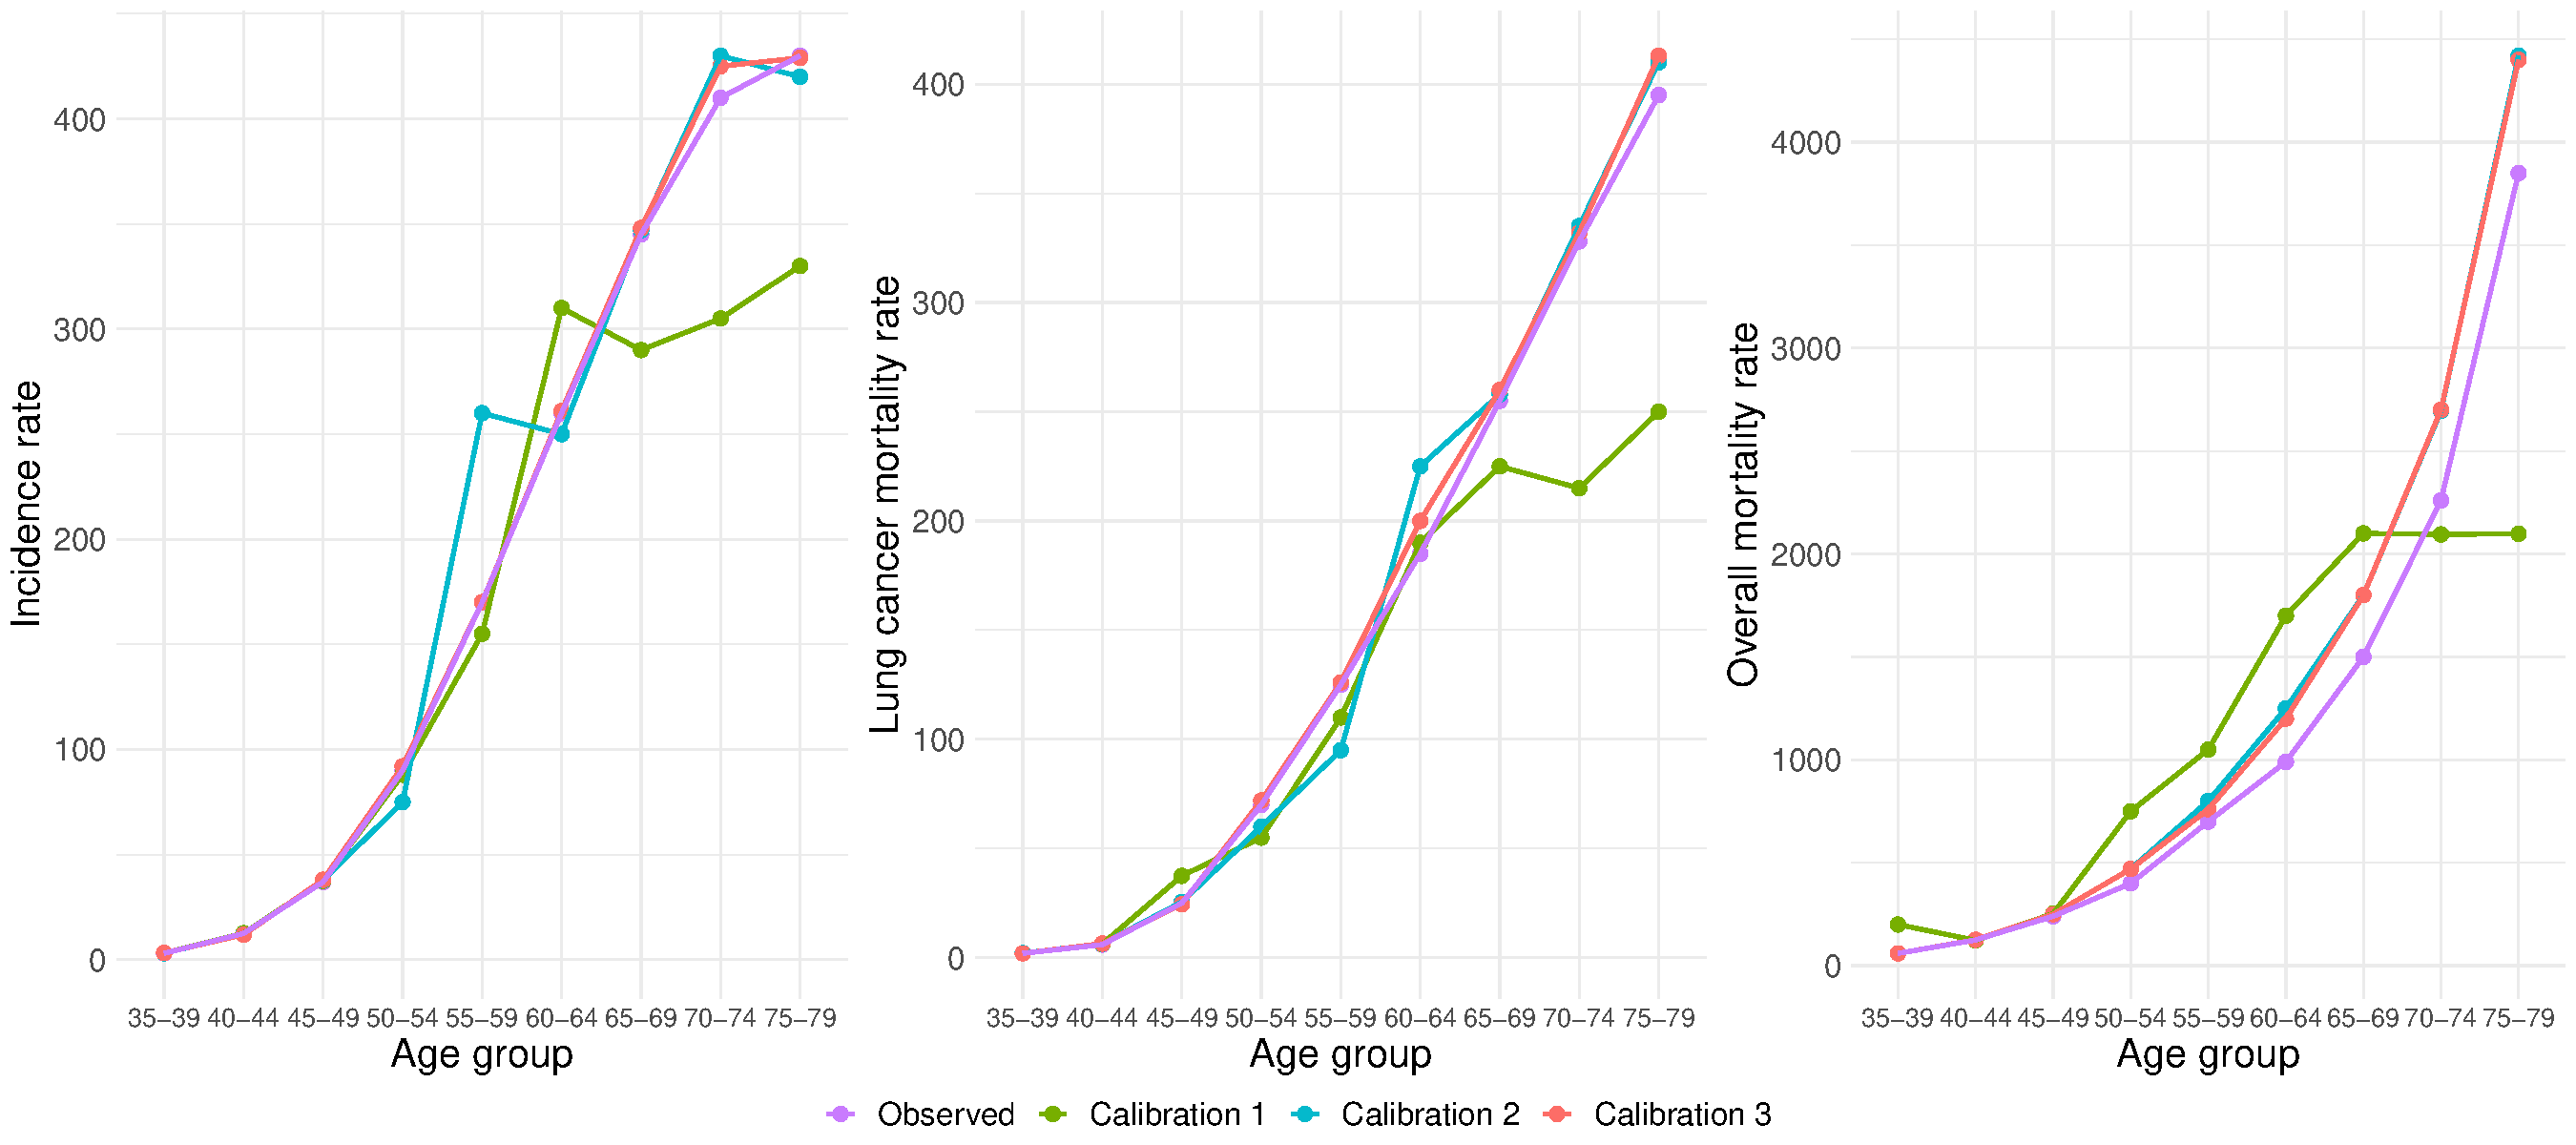
\includegraphics[width=\textwidth]{figs/calibration-curves.pdf}		
	\caption{Example of calibration curves for the lung cancer model}	
	\label{fig:calibration-curve}	
\end{figure}

\subsection{Optimization Methods}
In cost-effectiveness modeling, it is common to have an initial estimate of a good solution based on approximate values found in the scientific literature. For all optimization experiments conducted, a solution space of plus or minus $\pm 50\%$ was considered for each input variable, centered around this initial value.

First, we used different optimization methods to illustrate the performance differences between regular Bayesian Optimization and classical methods. For this purpose we used python implementations of commonly used methods: a hill-climbing technique (Nelder-Mead\cite{nelder-mead}), metaheuristics (Simulated Annealing (SA)\cite{simulated-annealing} and Particle Swarm Optimization\cite{pso}), and Bayesian Optimization with Gaussian Processes using Squared Exponential kernels (BO-SE). The default hyperparameter values were used for these methods, except for Particle Swarm Optimization, where the number of particles was set to 1,000 times the number of age groups calibrated.

We also developed an additional BO implementation with Gaussian Processes using the R programming language. This implementation was used as a rapid prototyping environment to evaluate different enhancements to the optimization process for our specific domain, without being too concerned by execution time. The acquisition function used is the Expected Improvement (equation \ref{eq:expected-improvement}, where $x^+$ represents the best optimum found so far), with Particle Swarm Optimization to search for its maximum. Finally, both SE kernels and OAK were implemented.

\begin{equation} \label{eq:expected-improvement}
	\begin{aligned}
		\text{EI}(x) &= \mathbb{E}[\max(f(x)-f(x^+), 0)]
	\end{aligned}
\end{equation}

Before starting the BO procedure we learn the lengthscales $l_1, ..., l_D$ and the variances $\sigma_0^1, \sigma_1^2, ..., \sigma_n^2$ of the OAK in a two stage process. In the first stage, we maximize the marginal likelihood for each lengthscale separately. In the second stage, we maximize the marginal likelihood for the whole set of variances.

\subsection{Stepwise calibration}
As an alternative to the conventional calibration we will also use a stepwise calibration approach. The rationale behind this method is that these simulation models follow a time-dependent sequential block layout. In this structure, the simulation output for a specific age group relies solely on the pertinent parameters for that age group and those preceding it, without being influenced by those of later age groups.

Let $f(p)$ denote the output of the complete simulation model with parameters $p = \{p_1, p_2, ..., p_n\}$ and let $k$ represent the number of age groups. We can make a partition $p^{(i)}$ of these parameters based on the age group $i$ they influence, such that $p = p^{(1)} \cup p^{(2)} \cup ... \cup p^{(k)}$ and $\underset{1\leq i \leq k}{\bigcap} p^{(i)} = \emptyset$. Using this partition and the output for each age group $s_i$, we can formulate the final output of the model $f(p) = s_k$ as a sequence of functions $f_i$:

\begin{equation} \label{eq:stepwise-function}
	\begin{aligned}
		s_1 &= f_1(p^{(1)})  \\
		s_2 &= f_2(p^{(2)} \mid s_1)= f_2(p^{(2)} \mid p^{(1)}) \\
		s_3 &= f_3(p^{(3)} \mid s_2)= f_3(p^{(3)} \mid p^{(1)} \cup p^{(2)}) \\
		&\dots \\
		f(p) = s_k &= f_k(p^{(k)} \mid s_{k-1})= f_k(p^{(k)} \mid p^{(1)} \cup p^{(2)} \cup \dots \cup p^{(k-1)}) \\
	\end{aligned}
\end{equation}	

The last term of each line is also conditional to the set of previous $f_i$, but they have been omitted from the notation for clarity purposes.

This decomposition allows a greedy approach where we can break down the calibration of the full model $f(p)$ into $k$ sequential tasks. This involves the iterative calibration of each age group, taking into account the previously calibrated parameter sets, as outlined in algorithm \ref{alg:stepwise}.

\begin{algorithm}[h!]
	\caption{Stepwise calibration with $k$ age groups}\label{alg:stepwise}
	\begin{algorithmic}
		\Require $\mathrm{target} \gets [t_1, \dots, t_k]$
		\For{$i \gets 1$ to $k$} \\
		%\State $p_*^{(i)} \gets \underset{p^{(i)}}{\mathrm{argmin}}\, \norm{f_i\left(p^{(i)} \mid p_*^{(1)}, \dots, p_*^{(i-1)}\right) -  t_i}$
		\State $p_*^{(i)} \gets \underset{p^{(i)}}{\mathrm{argmin}}\, \left\lVert f_i\left(p^{(i)} \hspace{0.25em} \bigg| \hspace{0.25em} \underset{j < i}{\bigcup} p_*^{(j)} \right) -  t_i \right\lVert$
		\EndFor
		\State \Return $[p_*^{(1)}, \dots, p_*^{(k)}]$
	\end{algorithmic}
\end{algorithm}

As expected from a greedy method, the optimum for each step does not guarantee being part of a global optimum, and each solution found by these calibration subtasks might potentially lead to suboptimal solutions in subsequent subtasks. On the other hand, this method reduces the complexity of the full calibration into $k$ smaller optimization problems, thereby reducing the overall computational effort required.

\section{Results}

\label{sec:results-partial}
\subsection{Partial calibration}
These results include a comparative performance analysis of BO versus other methods in calibrating simulation models for the initial four age groups. Figure \ref{fig:sim_times} illustrates the relationship between simulation time and calibration time for each method in this scenario. In instances where the models are extremely fast, the inference overhead of BO becomes dominant, and alternative methods achieve faster calibration by simulating the model multiple times. However, as we introduce an arbitrary delay in the simulation time to emulate larger simulation models, the Bayesian method's efficiency in the number of function evaluations results in faster calibration times. Specifically, for a simulation involving a single age group (with 11 parameters) and a simulation time exceeding 0.25 seconds, the Bayesian approach outperforms the alternative methods. We will refer to this time threshold as the critical simulation time.

In contrast, with the expansion of the problem's dimensionality the Bayesian method overhead increases significantly, as shown by the y-intercept in the same figure. While calibration times for other methods also increase, the critical simulation time experiences an exponential rise with the growing number of parameters, escalating from 0.2 seconds to 0.35, 0.95, and 3.25 seconds. The bottom left plot in figure \ref{fig:sim_times} projects that for all 9 age groups (99 parameters) BO-SE would be the fastest method only when each simulation demands more than 5 minutes of computation.

\begin{figure}[h!]
	\centering	
	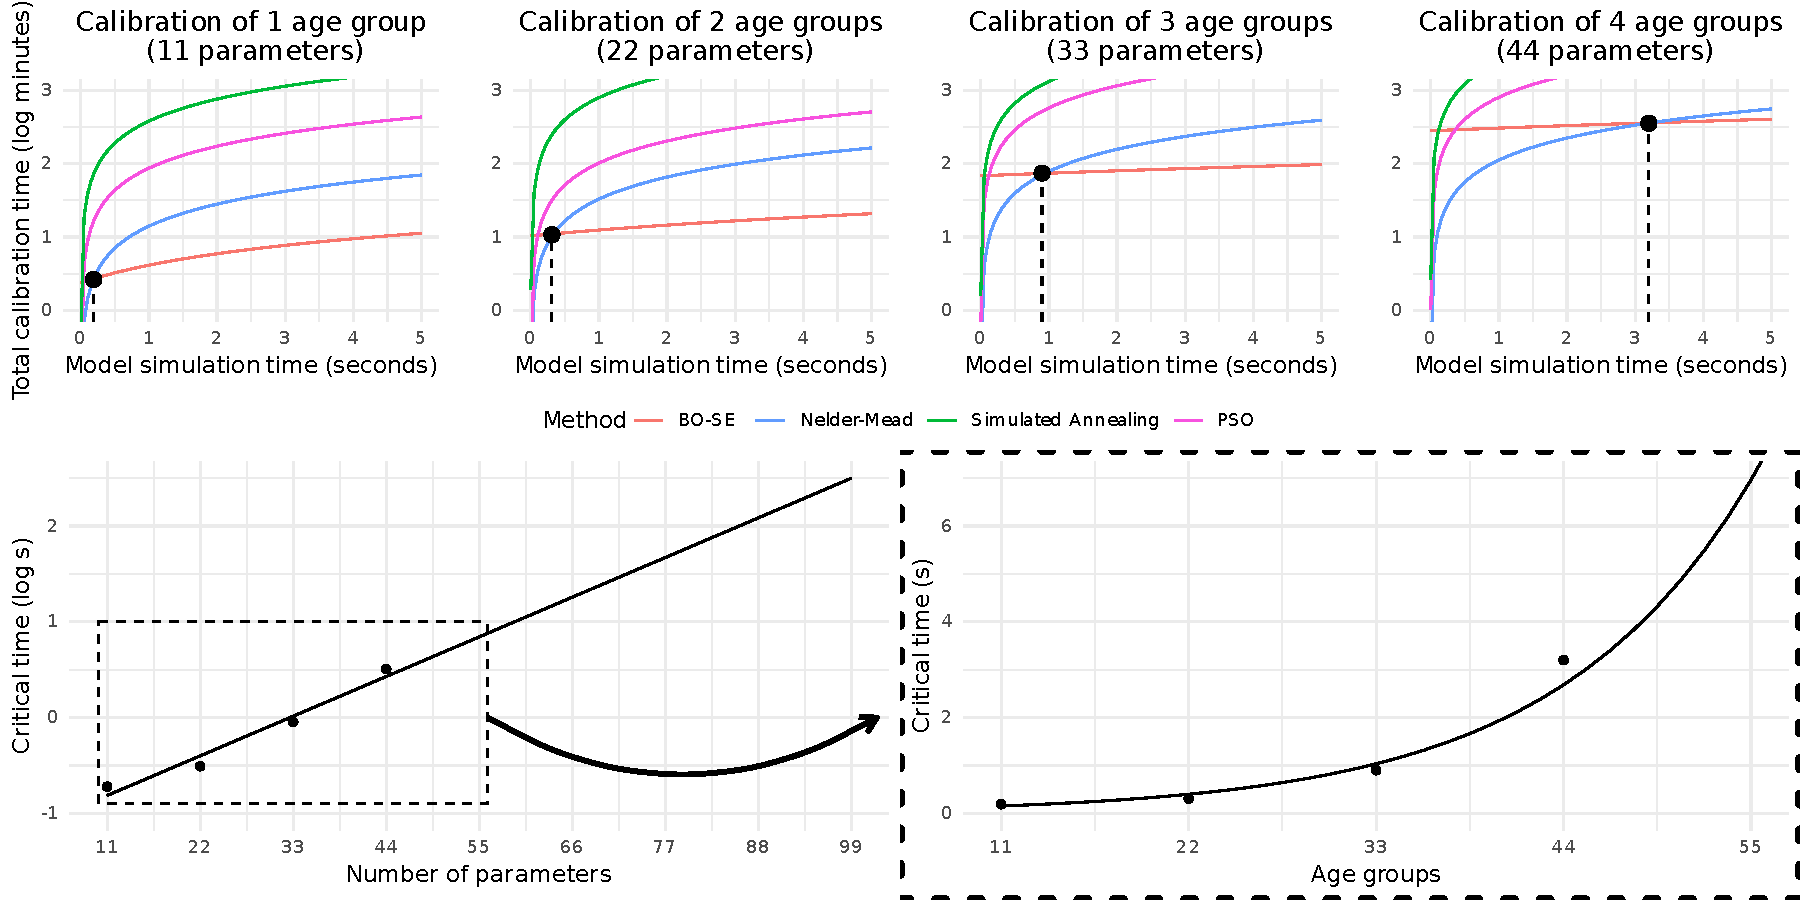
\includegraphics[width=\textwidth]{figs/crit_times_log.pdf}		
	\caption{Total calibration time in log scale against model simulation time (top) and the projected trend of the critical simulation time as a function of the number of parameters, in log scale (bottom left) and a zoomed-in area in linear scale (bottom right)}
	\label{fig:sim_times}	
\end{figure}

As expected from BO, we see a clear reduction in the number of evaluations when using BO to achieve a similar level of accuracy compared to other methods, as shown in figure \ref{fig:method_comparison}. Despite each iteration requiring a substantial amount of time due to the bayesian inference step, this overhead becomes less relevant as the simulation time of the model increases.

\begin{figure}[h!]
	\centering	
	\includegraphics[width=\textwidth]{figs/methods\_n1.pdf}		
	\caption{Lung cancer model calibration error by number of evaluations in logarithmic scale, simulating one age group}
	\label{fig:method_comparison}	
\end{figure}

In Figure \ref{fig:results_oak}, we present the median progression and interquartile range of the error throughout the optimization process, based on a sample of 30 random executions.  During the exploration of BO-OAK results, we identified a variable with substantial explanatory power on its own, which had the potential to yield misleading comparisons. To mitigate this concern, we introduced a third univariate SE kernel that exclusively considers this variable. This kernel demonstrated a lower average error and reduced spread compared to the regular SE kernel, owing to the simplified exploration of a smaller solution space with minimal information loss. However, it is noteworthy that OAK efficiently explores the entire 11-dimensional space, surpassing the average results of the univariate SE kernel while simultaneously reducing dispersion as the optimization progresses.

\begin{figure}[h!]
	\centering	
	\includegraphics[width=\textwidth]{figs/results\_q.pdf}		
	\caption{Median BO error with its interquartile range as the shaded area for the SE kernel (blue), the univariate SE kernel using only the most significant variable (green) and the OAK under a normality assumption for the inputs (red)}
	\label{fig:results_oak}	
\end{figure}

\subsection{Full calibration}
When applying the same methodology as outlined in section \ref{sec:results-partial} to consider the complete simulation for all nine age groups (i.e. 99 parameters), both BO methods cease to be viable calibration alternatives. They fail to identify satisfactory solutions even after several hours or days of computation, as indicated in table \ref{tab:calib-comparison}.

\begin{table}[h!]
	%\renewcommand{\arraystretch}{1.3}
	\begin{tabular*}{\textwidth}{@{\extracolsep\fill}p{15mm}rrrrrr}
		\toprule%
		& \multicolumn{2}{@{}c@{}}{\textbf{Calibration error}} & \multicolumn{2}{@{}c@{}}{\textbf{Number of evaluations}} & \multicolumn{2}{@{}c@{}}{\textbf{Calibration time}} \\\cmidrule{2-3}\cmidrule{4-5}\cmidrule{6-7}
		\multirow{-2}{*}{\textbf{Method}} & \fontsize{6pt}{6pt}\textbf{Conventional} & \fontsize{6pt}{6pt}\textbf{Stepwise} & \fontsize{6pt}{6pt}\textbf{Conventional} & \fontsize{6pt}{6pt}\textbf{Stepwise} & \fontsize{6pt}{6pt}\textbf{Conventional} & \fontsize{6pt}{6pt}\textbf{Stepwise} \\ \hline
		Nelder-Mead & 78.87 & 81.26 & 151,334 & 9,447 & 6min & 18sec \\
		%\rowcolor[HTML]{F0F0F0} 
		Simulated Annealing & 78.50 & 78.95 & 881,901 & 272,733 & 35min & 9min \\
		PSO & 87.76 & 83.04 & 243,450 & 518,656 & 11min & 36min \\
		%\rowcolor[HTML]{F0F0F0} 
		BO-SE & 1849.56 & 83.24 & 1,000 & 360 & 1d3h & 34min \\
		BO-OAK & 289.45 & 43.90 & 1,000 & 180 & 7d6h & 7h30 \\
		\botrule
	\end{tabular*}
	\smallskip
	\caption{Comparison of conventional vs stepwise calibration for the full simulation of all nine age groups}
	\label{tab:calib-comparison}	
\end{table}

Using stepwise calibration lowers the computational cost dramatically for BO, enabling the calibration for all nine age groups within a feasible timeframe while maintaining solutions of comparable quality. Furthermore, the critical simulation times are drastically reduced as well, as depicted in figure \ref{fig:crit-times-stepwise}. Notably, in a conventional calibration with BO-SE, the projected critical simulation time for the full model was approximately 300 seconds (see figure \ref{fig:sim_times}). In contrast, with a stepwise calibration, the critical time for the same method is reduced to 0.24 seconds.

\begin{figure}[h!]
	\centering	
	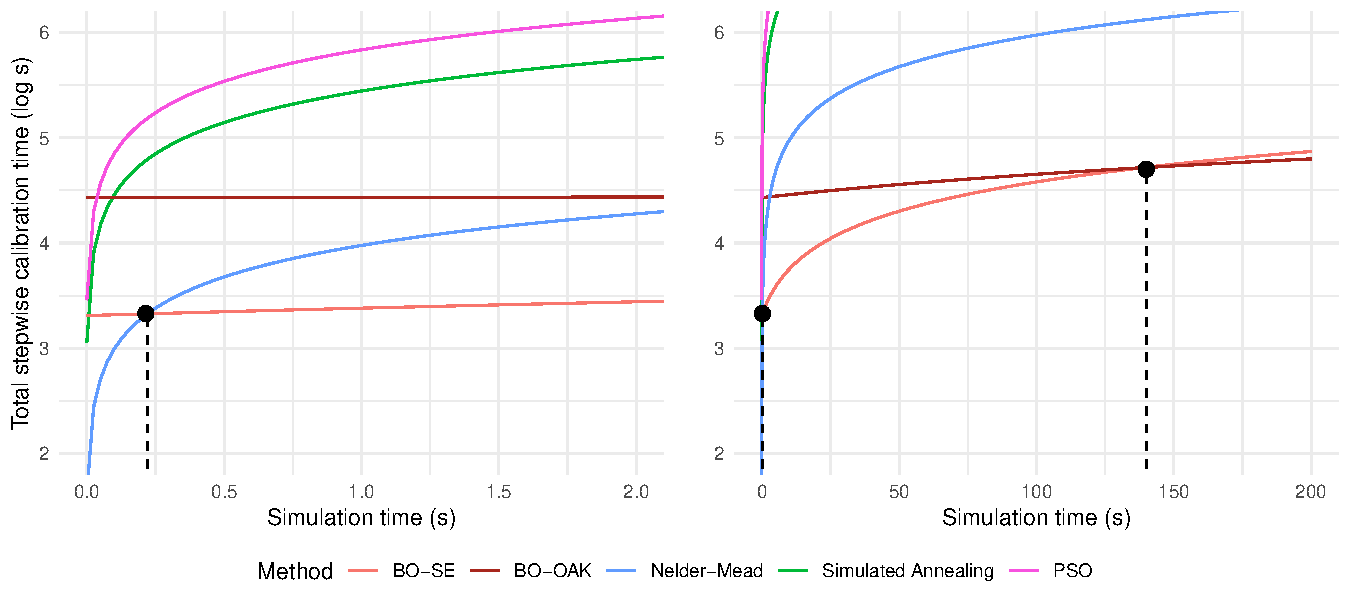
\includegraphics[width=\textwidth]{figs/crit_times_stepwise.pdf}		
	\caption{Total stepwise calibration time in a logarithmic scale against the full model simulation time, in two different x-axis scales to identify the BO-SE (left) and the BO-OAK (right) critical times}
	\label{fig:crit-times-stepwise}	
\end{figure}

Stepwise calibration not only achieves solutions for the simulation model with comparable error to those obtained by regular calibration but, in some cases, even lowers the error. In the case of BO-OAK, we observe a significant reduction in error for the first and last few age groups, with a slight increase in the middle ones. This indicates that the stepwise approach manages to find a better overall solution (see table \ref{tab:calib-comparison} and figure \ref{fig:stepwise-error}).

It is important to note a sharp increase in error observed in the seventh age group, a phenomenon shared among all methods. This increase is attributed to the nature of the simplified simulation utilized and the manner in which the target has been selected. Consequently, it is crucial to recognize that this effect is a limitation inherent in the simulation model and not a shortcoming of the optimization process.

\begin{figure}[h!]
	\centering	
	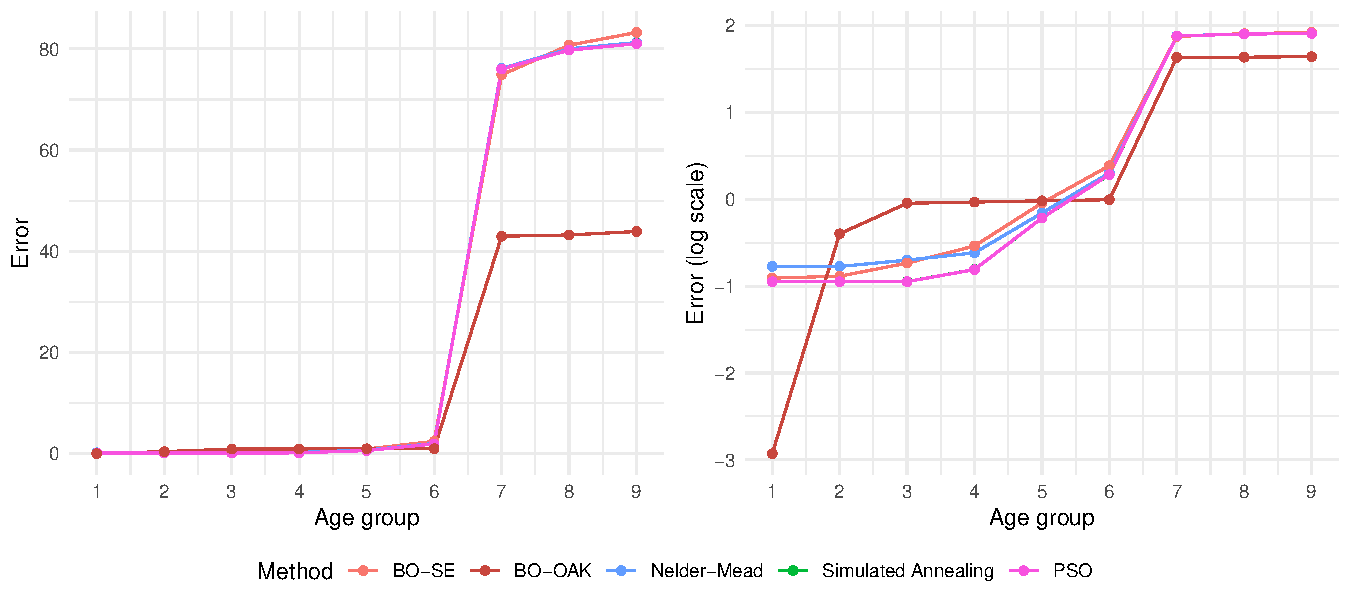
\includegraphics[width=\textwidth]{figs/stepwise_error.pdf}		
	\caption{Stepwise calibration error for each age group in linear scale (left) and logarithmic scale (right)}
	\label{fig:stepwise-error}	
\end{figure}

\section{Discussion}
BO is currently regarded as a state-of-the-art optimization method in various domains that involve costly functions to evaluate. When the computational cost of the objective function is large enough, Bayesian Optimization might be the natural choice. In this work, the tested simulation model was intentionally designed to be computationally inexpensive, allowing traditional calibration methods to work efficiently within a reasonable time. However, to emulate and extrapolate the results to larger models, artificial delays were introduced in the simulation. This extension of the analysis allowed for the exploration of scenarios with arbitrary simulation times, revealing the circumstances where Bayesian methodology could offer significant advantages.

The initial bottleneck in the optimization process is centered around optimizing the acquisition function, particularly when the number of observations is small enough that surrogate model regression is not yet a significant problem. Since the search space remains constant, the optimization of the acquisition function doesn't become significantly more expensive as more data is observed.

Concerning surrogate model regression, Gaussian processes with Squared Exponential (SE) kernels encounter significant challenges due to the curse of dimensionality. In high-dimensional problems, the number of observations required to explore the solution space rapidly increases, making regression impractical when attempting to invert large matrices to calculate the posterior predictive distribution. To tackle this challenge, OAK helps reduce the number of necessary observations, alleviates the impact of expanding matrices, and improves the efficiency of the search process. The scaling issues observed in figure \ref{fig:sim_times}, attributed to increasing dimensionality, emphasize the need for high-dimensional enhancements such as OAK.

Another complementary way to avoid these scaling issues is to use stepwise calibration. Using this technique allows us to calibrate models that are prohibitive using other methods by reducing a high number of parameters to a sequence of calibration tasks with fewer parameters. Stepwise calibration is a sensible choice to use when the target function has a sequential block structure, but even if each step makes an optimal choice it does not guarantee that the global solution built from those is optimal as well. We are confident in the suitability of this technique for simulation models used in cost-effectiveness analysis for two reasons. First, the solutions found in our tests have a similar error to those found using conventional calibration. In some cases the solutions are even better than the traditional approach, as observed with BO-OAK. Second, the tuned OAK hyperparameters assign a negligible weight to the orders of interaction greater than one. This suggests that the interaction between parameters is not overly complex, making the stepwise approach a reasonable approximation for problems where only the first few orders of interaction are important\cite{gp-additive}. The stepwise methodology presented here can be generalized and applied in other sequential block problems with similar properties.

The results strongly indicate that stepwise calibration represents a significant improvement over conventional calibration. However, it is crucial to adapt the optimization method used during calibration to the model simulation time, as illustrated by the critical times in Figure \ref{fig:crit-times-stepwise}. To illustrate this point with the results from this work, three possible scenarios are listed in table \ref{tab:crit-times-stepwise}.

\begin{table}[h!]
	%\renewcommand{\arraystretch}{1.3}
	\begin{tabular*}{.75\textwidth}{@{\extracolsep\fill}rc}
		\textbf{Model simulation time} & \textbf{Fastest stepwise calibration method} \\ \hline
		\textless{}0.24s & Nelder-Mead \\
		0.24s - 140s & BO-SE \\
		\textgreater{}140s & BO-OAK
	\end{tabular*}
	\smallskip
	\caption{Fastest optimization method according to model simulation time, as seen in figure \ref{fig:crit-times-stepwise}}
	\label{tab:crit-times-stepwise}	
\end{table}

In particular, BO-OAK and stepwise calibration can be combined with impressive results. The stepwise approach greatly benefits BO, successfully overcoming its inherent poor dimensional scalability. This combination leads to a faster discovery of better solutions than the rest of methods as long as the simulation model is moderately time-consuming ($\sim 2$ minutes). Notably, these results are achieved despite using a basic BO-OAK implementation, suggesting that further improvements in the kernel numerical computation could substantially enhance the calibration process, reducing the critical time even further.

Lu et al\cite{gp-additive-orthogonal} mention that an interesting direction of work would be to extend OAK to Bayesian Optimization leveraging the inferred low-order representation. In our tests we show that, even with a straightforward application of OAK on this simple example, a slight improvement over the SE kernel is noticeable. This improvement is expected to be more meaningful for complex models, where more structure can be leveraged. It is noteworthy that these results hold even though some assumptions of the model were not met. Specifically, hyperparameter tuning was performed with a dataset sampled from a uniform input distribution, while the constrained kernels were calculated assuming normality in the input. Even if these distributions were consistent, we still would have the problem of determining the input distribution for the actual optimization process, which would be neither normal nor uniform.

%gp max likelihood ill-posed -> impose gaussian noise

\section{Future Work and Conclusions}
An aspect not covered in this article is constraint handling. Simulation models, being often highly constrained problems, provide another layer of the solution space structure that can be leveraged to enhance the calibration process. Extensive literature exists on this topic, exploring the use of additional surrogate models or novel acquisition functions\cite{gp-constraints}. While some of these methods assume independent constraints, it's worth noting that simulation models in cost-effectiveness analysis often involve interdependent constraints. Nevertheless, studies indicate that the independence assumption tends to work well in practice in many cases \cite{bo-constraint-dependence}.

We also mentioned in the discussion the convenience of exploiting the parallelization potential of the different areas of the optimization process. For that purpose we use the Particle Swarm method for the optimization of the acquisition function, but other more sophisticated venues for parallelization include batched optimization\cite{gp-batch}, parallel acquisition functions\cite{gp-parallel-acq-func} or GPU approaches\cite{gp-gpu} among others.


\section*{Declarations}
\subsection*{Funding}
This work was supported by a grant from the Instituto de Salud Carlos III-ISCIII (Spanish Government) co-funded by European Regional Development Fund, a way to build Europe (CIBERESP CB06/02/0073, PI19/01118), also with the support of the Secretariat for Universities and Research of the Department of Business and Knowledge of the Government of Catalonia. Grants to support the activities of research groups (SGR 2017–2021). Grant number 2021SGR1029. We thank the CERCA Programme and Generalitat de Catalunya for institutional support.
\subsection*{Financial interests}
All authors certify that they have no affiliations with or involvement in any organization or entity with any financial interest or non-financial interest in the subject matter or materials discussed in this manuscript.
\subsection*{Ethics approval}
Not applicable
\subsection*{Consent to participate}
Not applicable
\subsection*{Consent for publication}
Not applicable
\subsection*{Availability of data and materials}
Not applicable
\subsection*{Code availability}
The code for the optimization methods used in this work are available in the following links:
\begin{itemize}
	\item{Nelder-Mead: \\ \url{https://docs.scipy.org/doc/scipy/reference/optimize.minimize-neldermead.html}}
	\item{Simulated Annealing: \\ \url{https://docs.scipy.org/doc/scipy/reference/generated/scipy.optimize.dual_annealing.html}}
	\item{PSO: \\ \url{https://pyswarms.readthedocs.io/en/latest/}}
	\item{BO (python): \\ \url{https://secondmind-labs.github.io/trieste/1.1.2/index.html}}
	\item{BO (R): \\ \url{https://github.com/david-gomez-guillen/stepwise-calibration}}
\end{itemize}

The lung cancer simulation model used is part of an independent project and its code is not publicly available. If needed, the authors of the original article\cite{lung-model} can be contacted at mireia@iconcologia.net.

\subsection*{Authors' contributions}
Following the CRediT taxonomy (\url{https://credit.niso.org/}), the authors contributions are listed below:
\begin{itemize}
	\item David Gómez-Guillén: conceptualization, methodology, software, validation, formal analysis, investigation, writing-original draft preparation, visualization
	\item Mireia Diaz: conceptualization, writing-review and editing, visualization, supervision, project administration, funding acquisition
	\item Josep Lluís Arcos: supervision, project administration
	\item Jesus Cerquides: conceptualization, writing-review and editing, visualization, supervision, project administration
\end{itemize}

\bibliography{sn-bibliography}% common bib file
%% if required, the content of .bbl file can be included here once bbl is generated
%%\input sn-article.bbl

\end{document}
